\section{Evaluation}\label{sec:eval}

\begin{figure}
  \centering
  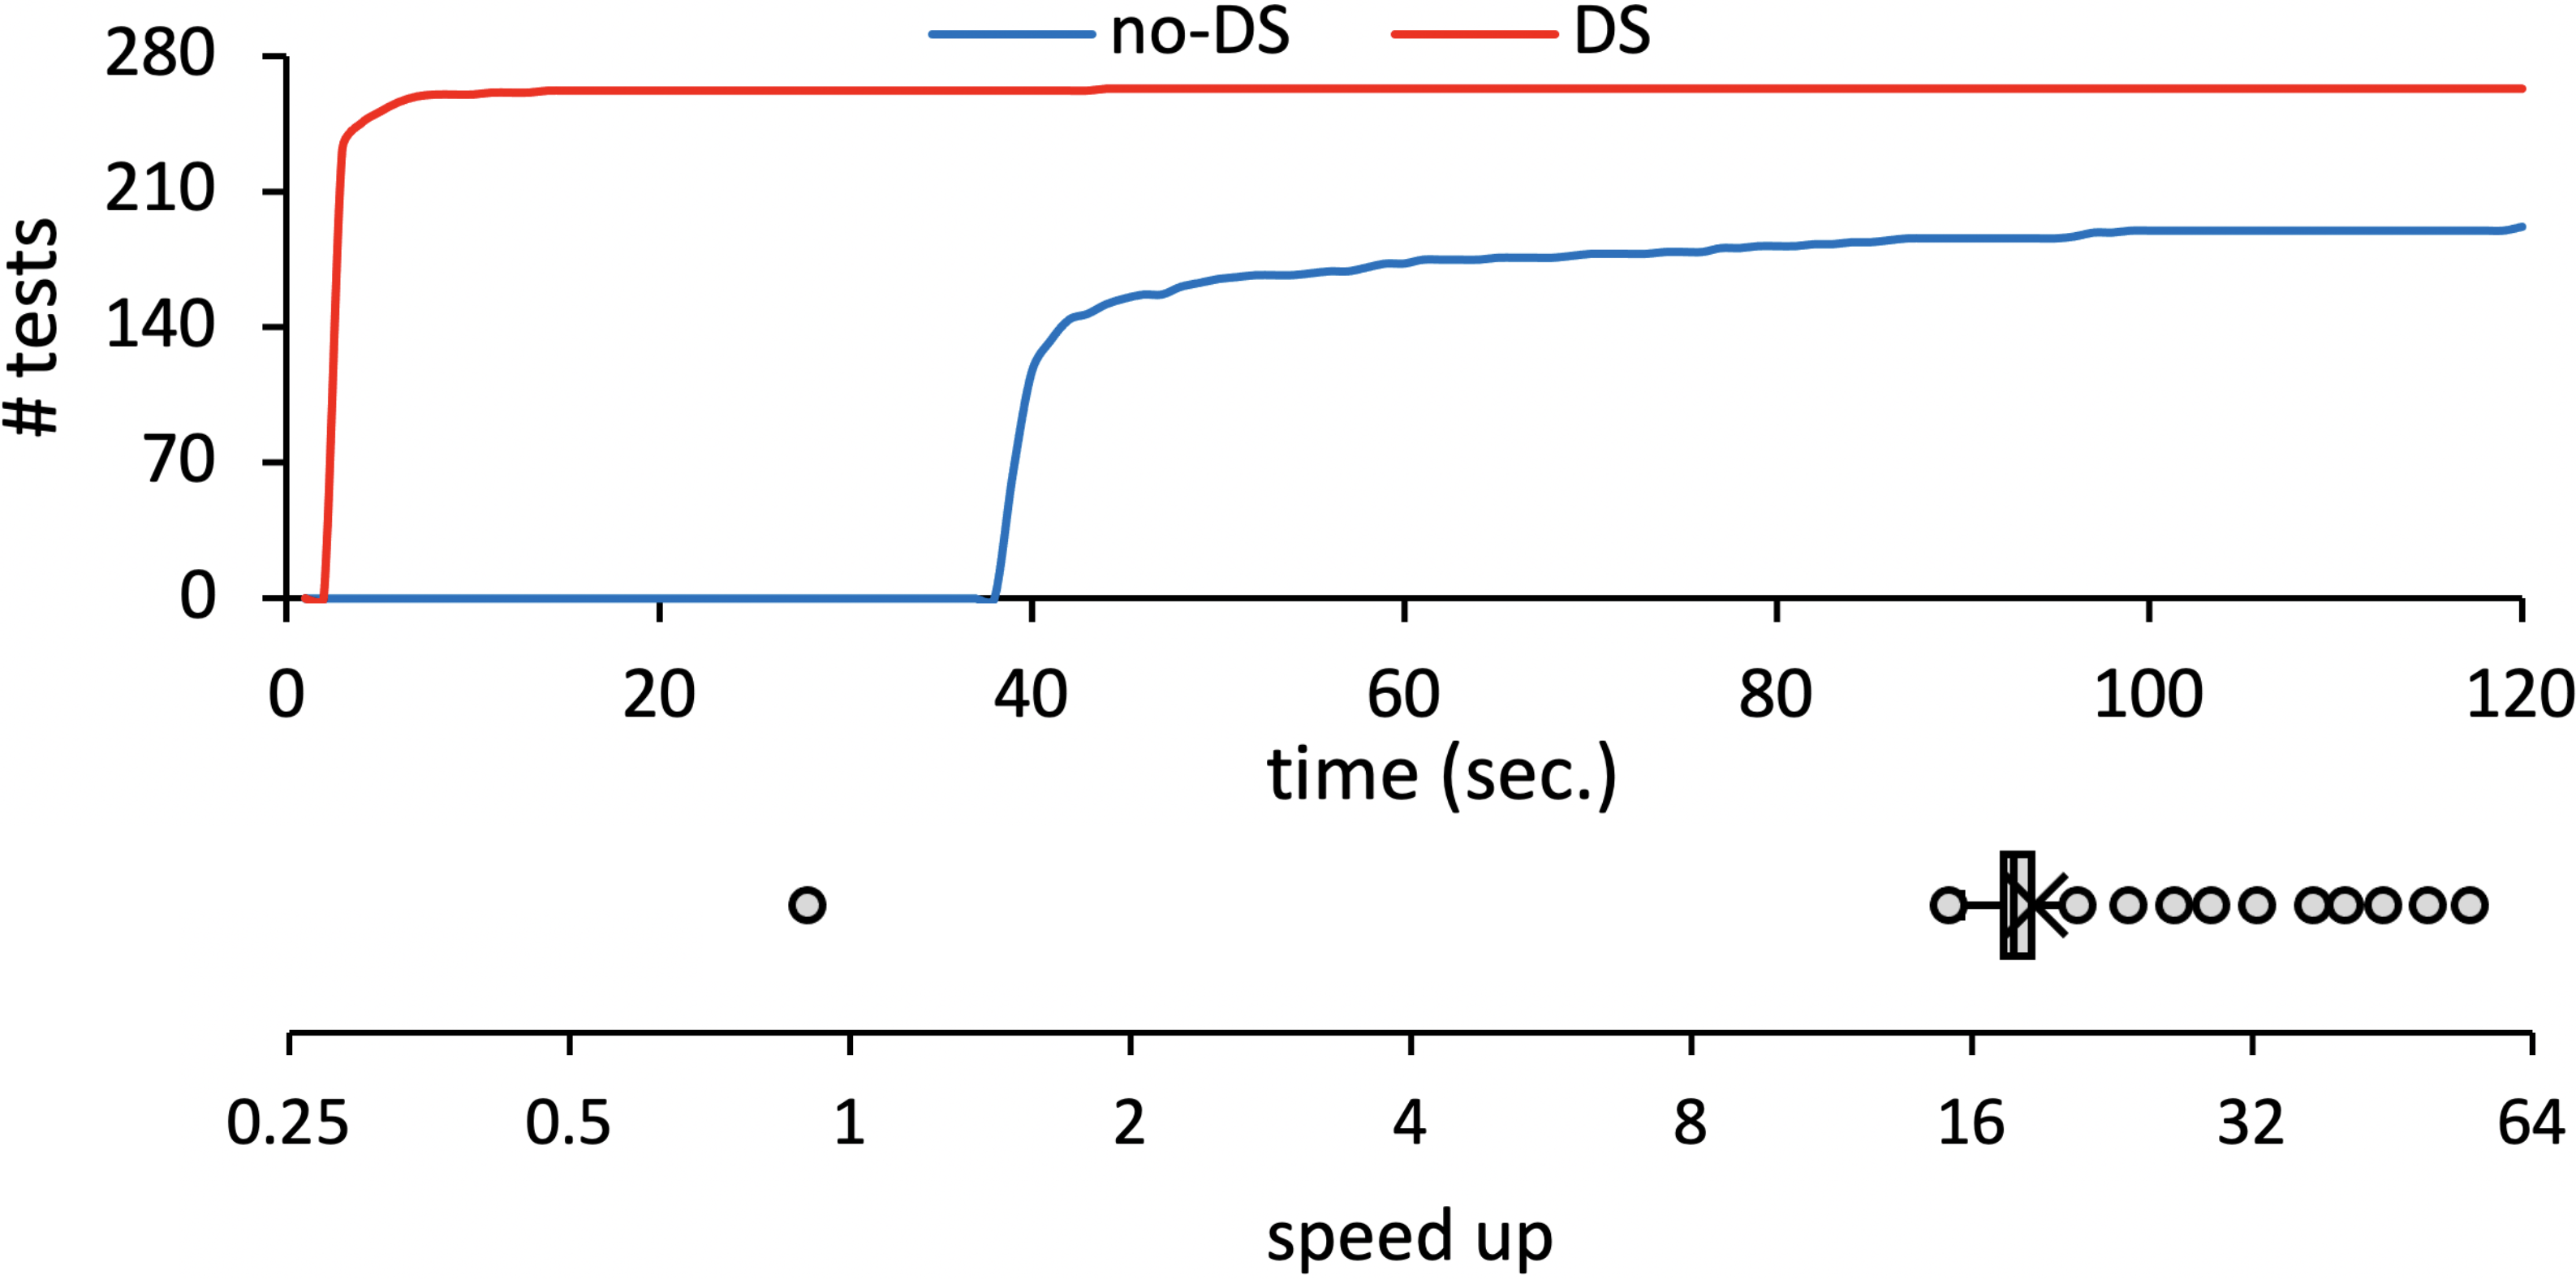
\includegraphics[width=\linewidth]{img/conc-analysis-time}
  \vspace*{-1.5em}
  \caption{Analysis time for Lodash 4 tests with (DS) and without (no-DS) the
  dynamic shortcut within 5 minutes.}
  \label{fig:conc-analysis-time}
  \vspace*{-1.5em}
\end{figure}

We evaluated our tool based on the following research questions:
\begin{itemize}
  \item \textbf{RQ1) Analysis Speed-up:} How much analysis time is reduced by
    adding dynamic shortcut to static analysis?
  \item \textbf{RQ2) Precision Improvement:} How much analysis precision is
    improved by replacing the manual modeling with dynamic shortcut?
  \item \textbf{RQ3) Opaque Function Coverage:} How many opaque functions are
    covered by dynamic shortcut without using manual modeling?
\end{itemize}
We targeted the official 306 tests of Lodash 4
(v.4.17.20)\footnote{https://github.com/lodash/lodash/blob/4.17.20/test/test.js}
used in motivating examples (Section~\ref{sec:motivation}).  The most recent
papers for JavaScript static analysis techniques~\cite{value-refinement,
value-partitioning} also evaluated their techniques based on them.
Among them, we filtered out \inred{37} tests including JavaScript language
features SAFE does not support, such as dynamic code generation using
\jscode{Function}, getter/setter, and browser specific features
(e.g. $\jscode{__proto__}$).  Thus, we only targeted \inred{269} out of 306
tests for the evaluation.  We performed our experiments on an Ubuntu machine
equipped with 4.2GHz Quad-Core Intel Core i7 and 64GB of RAM.


\subsection{Analysis Speed-up}

\begin{figure}
  \centering
  \begin{subfigure}[t]{0.48\textwidth}
    \vspace*{-1em}
    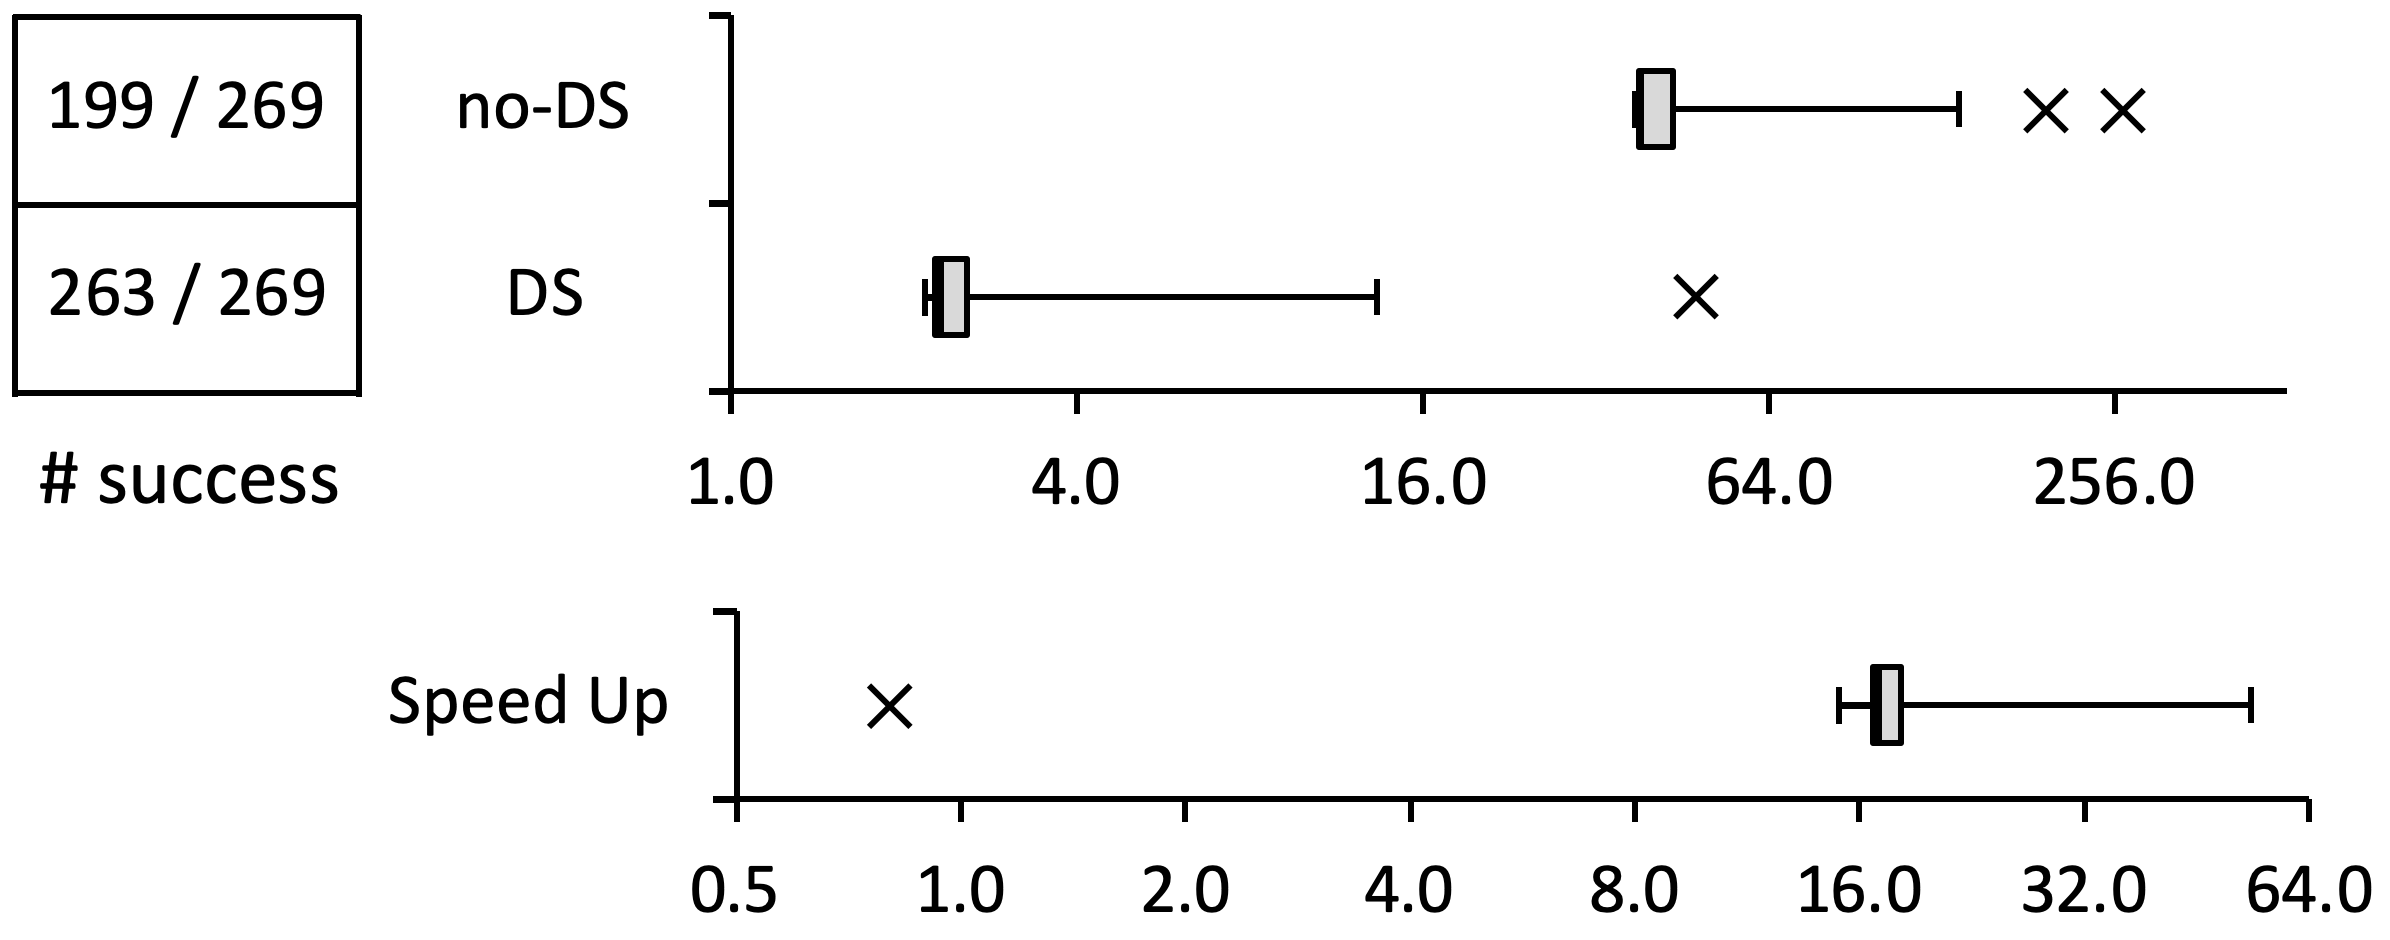
\includegraphics[width=\linewidth]{img/abs-analysis-time}
    \caption{Analysis time and speed up.}
    \label{fig:abs-time-speed}
  \end{subfigure}
  \begin{subfigure}[t]{0.48\textwidth}
    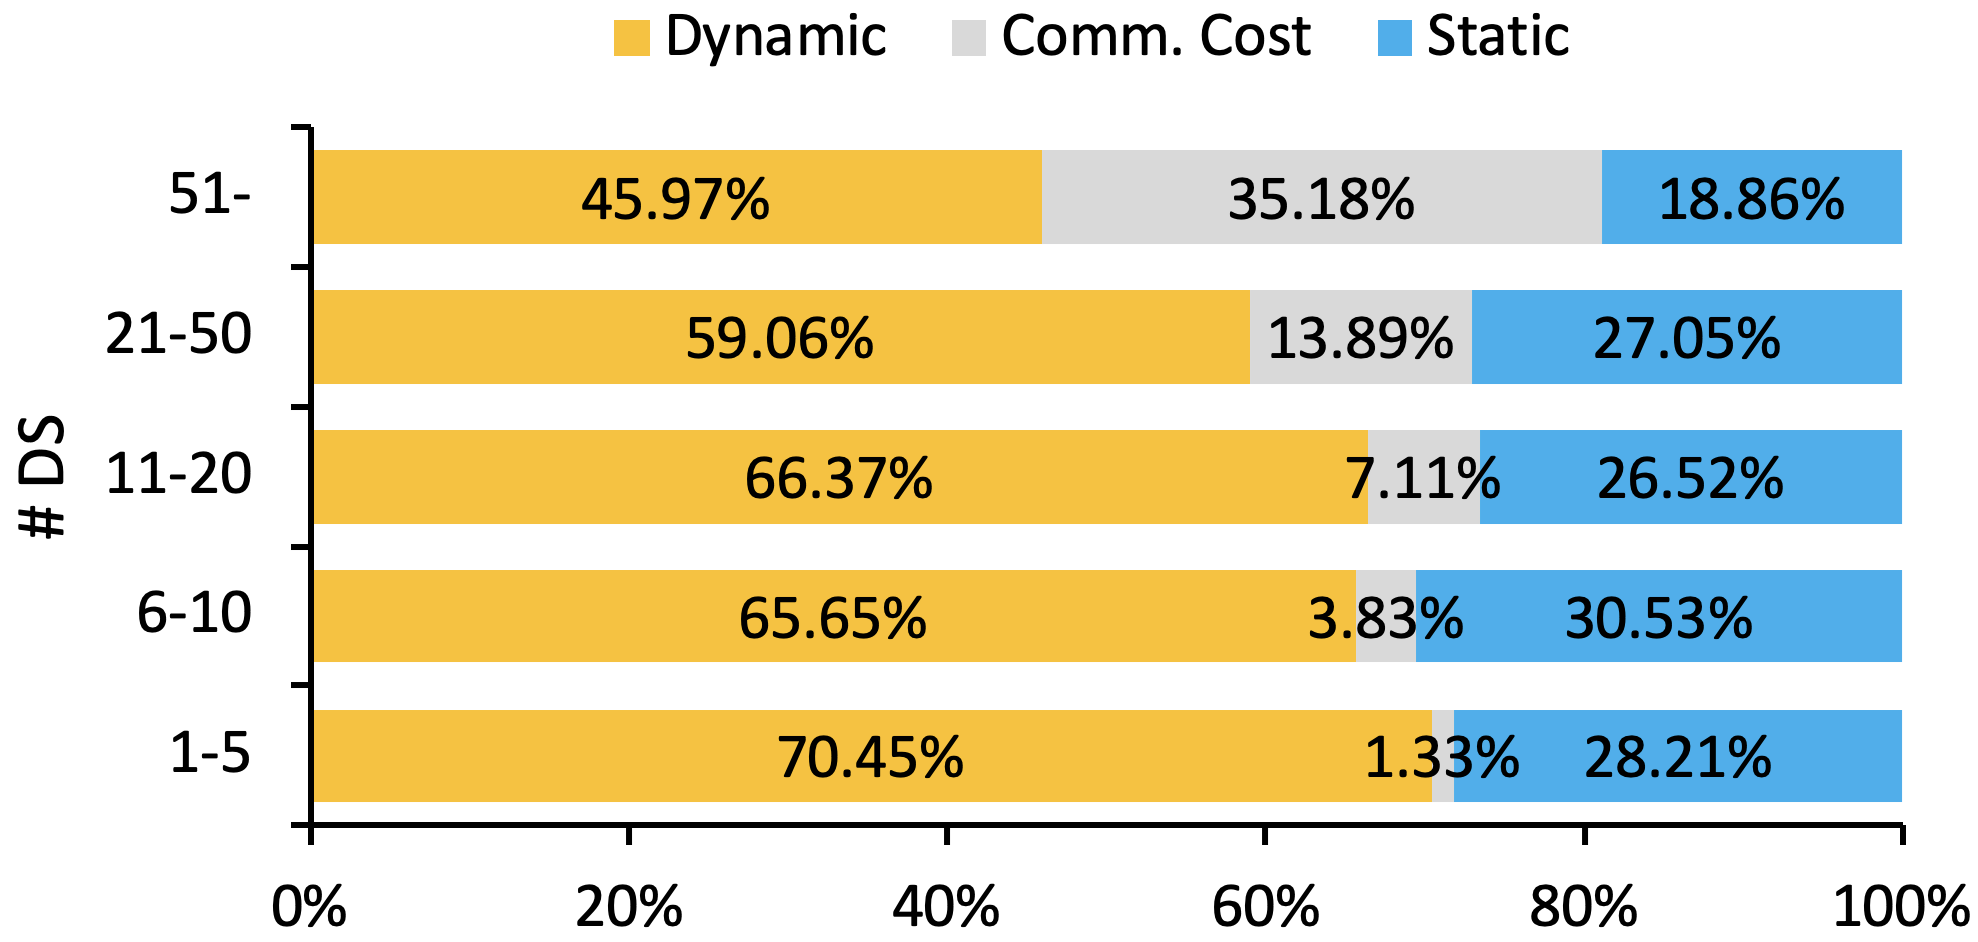
\includegraphics[width=\linewidth]{img/abs-analysis-ratio}
    \caption{Analysis time ratio.}
    \label{fig:abs-analysis-ratio}
  \end{subfigure}
  \caption{Analysis time for abstracted Lodash 4 tests with (DS) and without
  (no-DS) the dynamic shortcut within 5 minutes.}
  \label{fig:abs-analysis-time}
  \vspace*{-1.5em}
\end{figure}

To evaluate the effectiveness of the dynamic shortcut, we performed static
analysis for \inred{269} Lodash 4 tests with and without dynamic shortcut.
Figure~\ref{fig:conc-analysis-time} depicts the box plot chart for their
analysis time and for speed up after applying the dynamic shortcut.  While the
base analysis (no-DS) finished \inred{199} out of \inred{269} tests within 5
minutes, our tool finished all tests with the dynamic shortcut (DS).  For
\inred{199} tests analyzable by both analyses, the analysis (no-DS) took
\inred{168.4} seconds and \inred{12.2} seconds on average without dynamic
shortcut (no-DS) and with dynamic shortcut (DS), and the dynamic shortcut
accelerates \inred{20.16}\textsf{x} the static analysis on average.  Only for
one test using $\jscode{_.sample}$ (a Lodash 4 library that randomly samples a
value from a given array), the static analysis using dynamic shortcut had
\inred{0.81}\textsf{x} speed of the base analysis because of the frequent use of
dynamic shortcut (\inred{24} times).

Unfortunately, since most of Lodash 4 tests use concrete values instead of
non-deterministic user inputs, they could be analyzed via a few number of
dynamic shortcut.  In fact, among \inred{269} tests, \inred{262} tests analyzed
via a single usage of dynamic shortcut without using abstract semantics.
However, the arguments of library functions might include non-deterministic user
inputs in the real-world JavaScript programs.  Thus, we modified Lodash 4
official tests with abstract values to mimic the use patterns of library
functions.  We randomly selected literals and replace subset of them to their
corresponding typed abstract values.  For example, if we pick a numerical
literal \jscode{42}, we modified it to the abstract numeric value
$\top_{\code{num}}$, which represents the all numerical values.  In the
remaining section, we evaluated our tool based on the randomly abstracted tests
of Lodash 4.

\todo


\subsection{Precision Improvement}

\begin{figure}
  \centering
  \begin{subfigure}[t]{0.48\textwidth}
    \vspace*{-1em}
    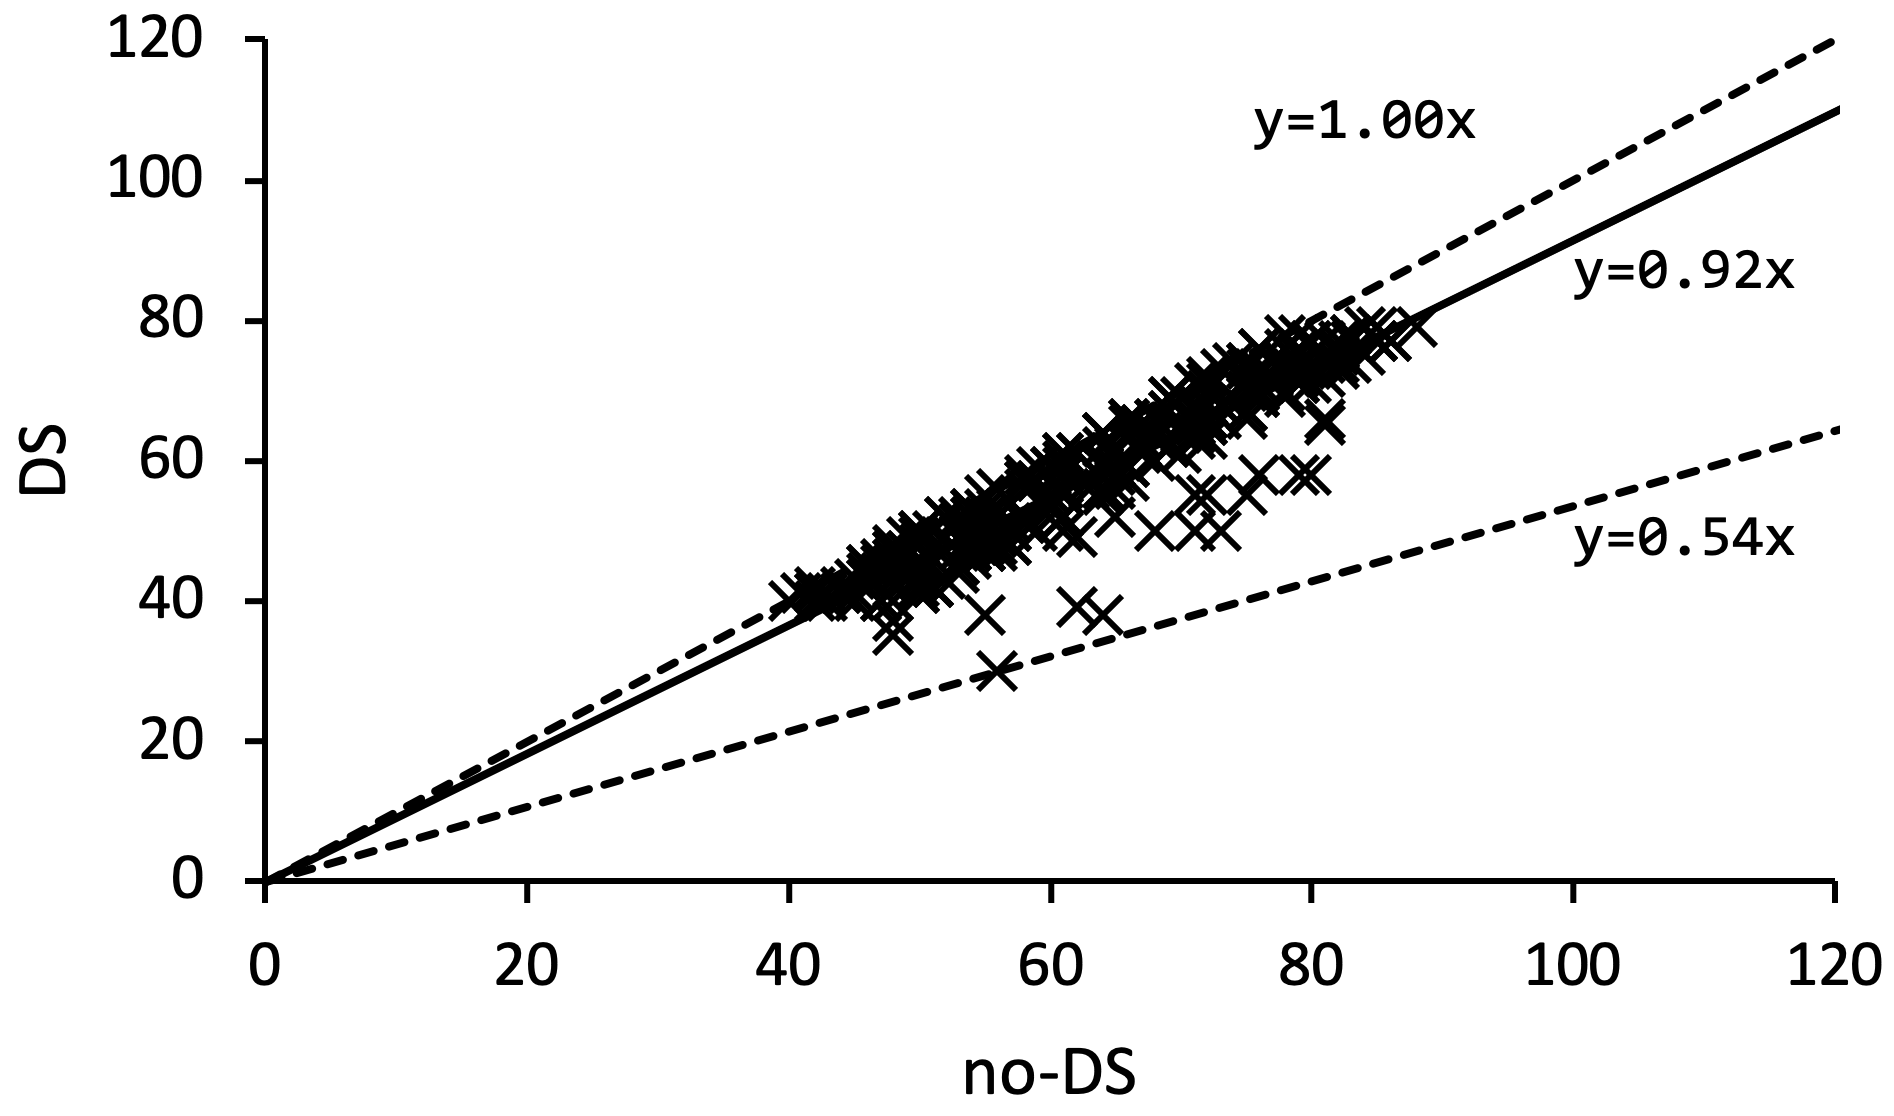
\includegraphics[width=\linewidth]{img/precision-func}
    \caption{Reachable functions.}
    \label{fig:precision-func}
  \end{subfigure}
  \begin{subfigure}[t]{0.48\textwidth}
    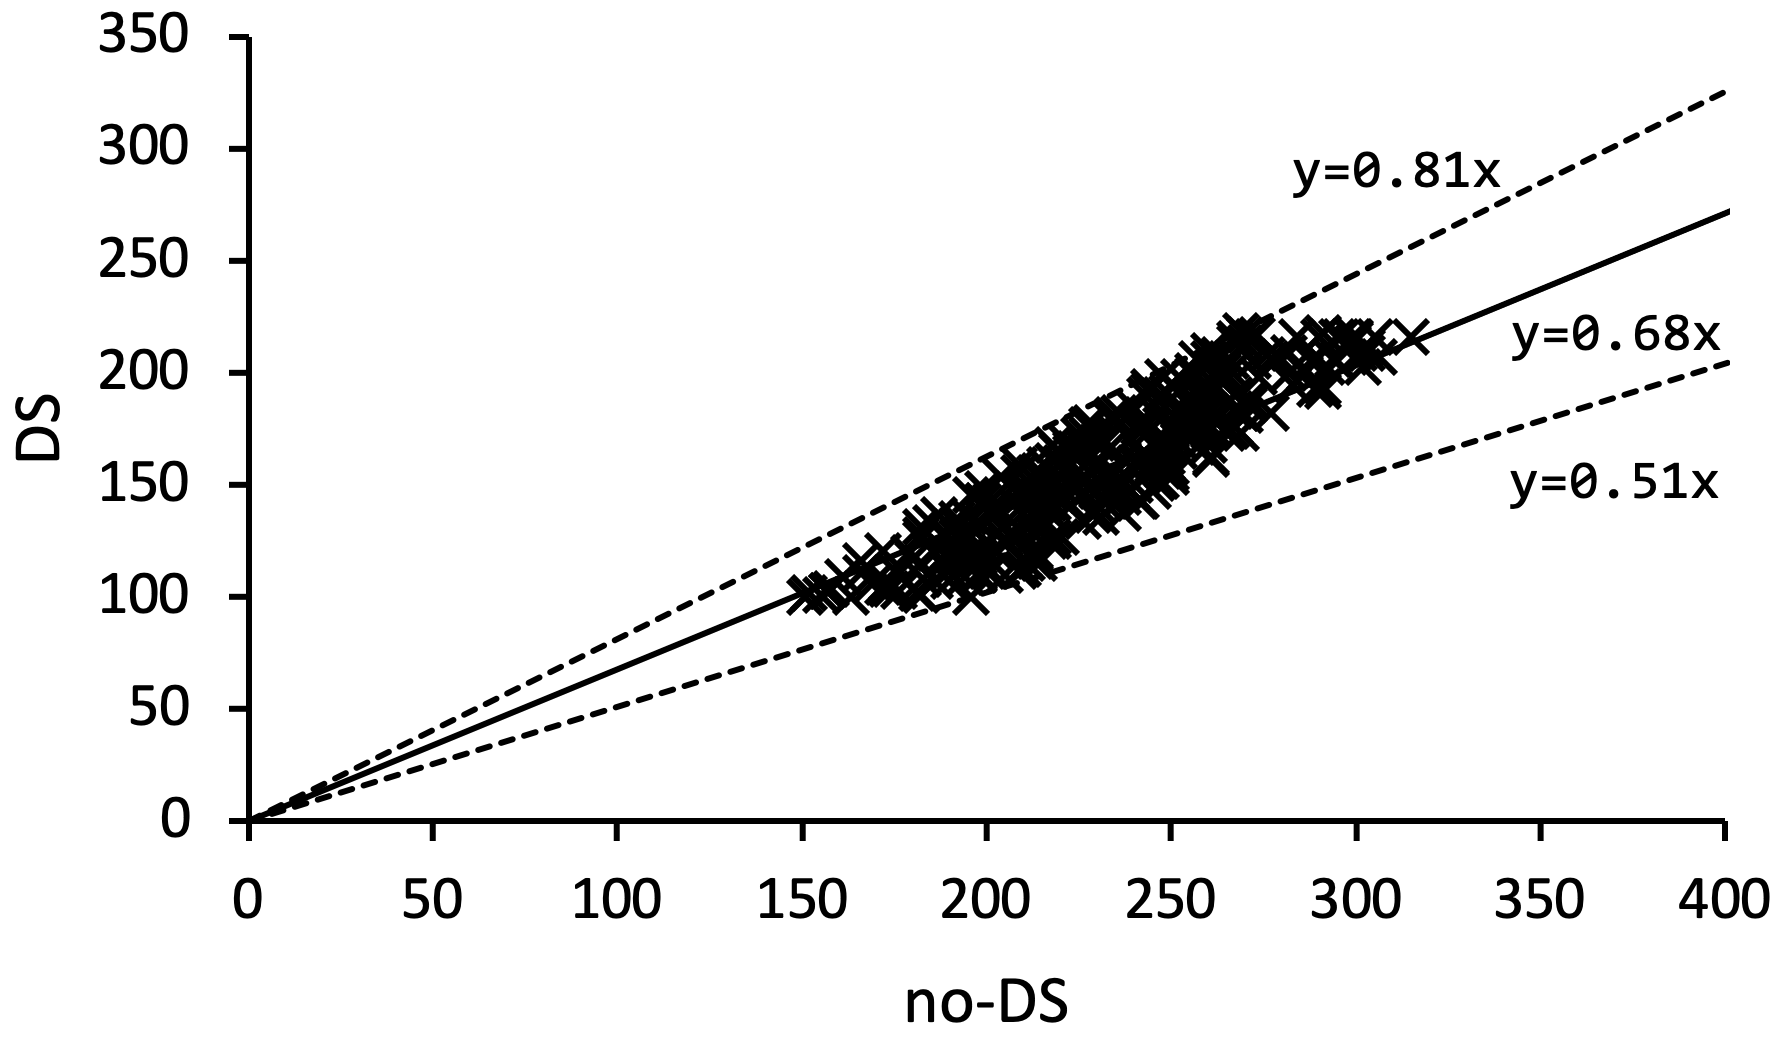
\includegraphics[width=\linewidth]{img/precision-branch}
    \caption{Reachable branches.}
    \label{fig:abs-analysis-ratio}
  \end{subfigure}
  \caption{The comparison of analysis precision with (DS) and without (no-DS)
  dynamic shortcut}
  \label{fig:precision}
  \vspace*{-1.5em}
\end{figure}

\todo


\subsection{Opaque Function Coverage}

\todo
